\begin{figure}[htpb!]
\centering
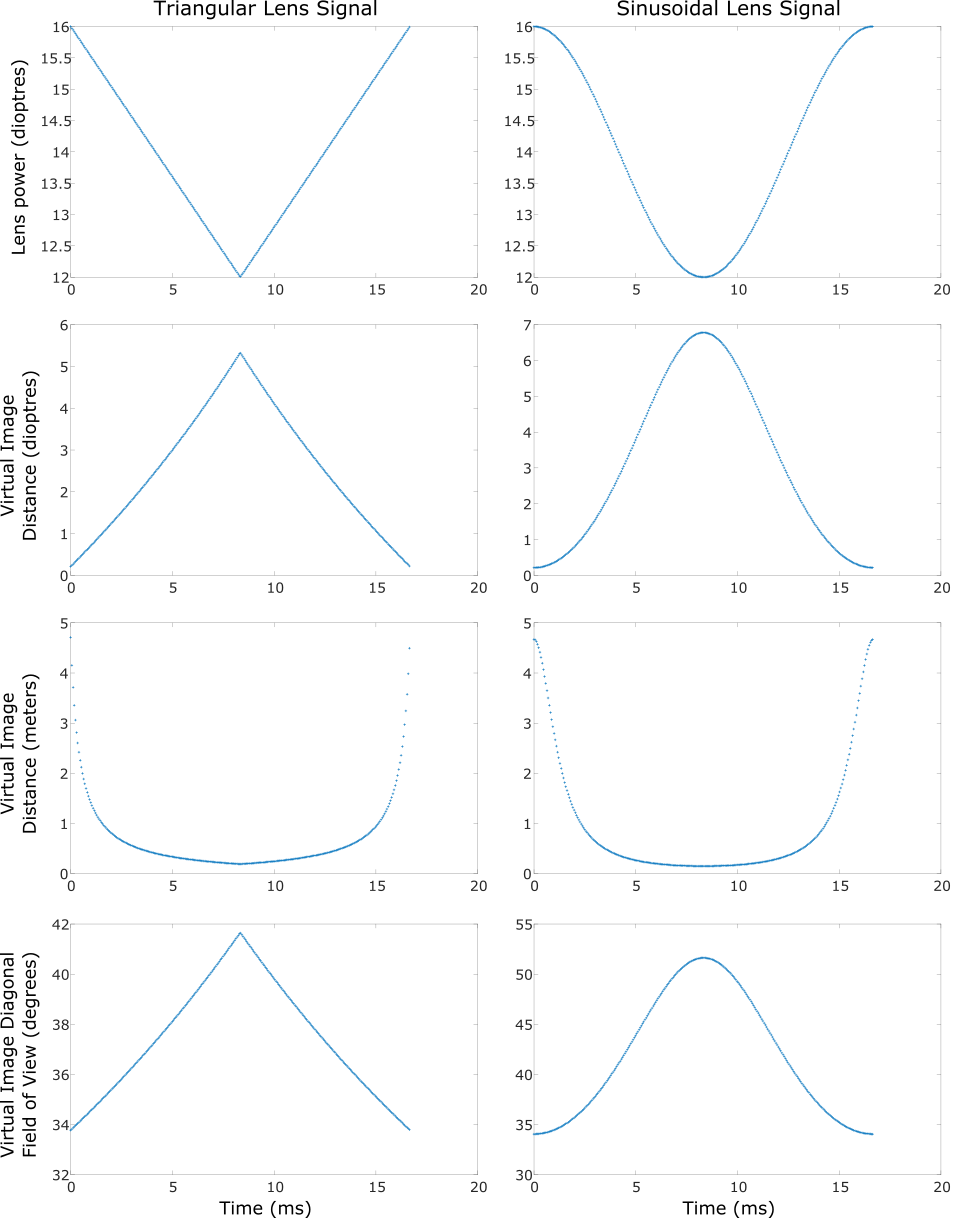
\includegraphics[width=0.9\textwidth]{images/volumetric/graphs}
\caption[Volumetric NED: Modelling depth and field of view of display's depth planes]{Graphs modeling the depth distribution and FoV of the displayed single-color binary images that compose the volume formed by synchronizing the DMD projector and a continuously oscillating focus-tunable lens. The oscillating lens's optical power can follow a triangular waveform \emph{(Left column)} or a sinusoidal waveform \emph{(Right column)}. Data presented in these graphs are used in the rendering pipeline to convert 3-D scene information to multiple single-color binary images that are displayed by the NED. Equations used to generate these graphs are described in Section~\ref{sec:volumetric:Optical_design}.}
\label{fig:volumetric:graphs}
\end{figure}


